\chapter{Synchronization Plugins}
Synchronization Plugins are modules which provides access to a certain device,
application or protocol. All of those plugins provide independent of the
synchronized content/format or connection type, the same functions:
\begin{itemize}
\item initialize. This function parse the plugin configuration and initializes
the plugin. If the plugin acts as server, it also initializes this one and 
listen for incoming connections.
\item finalize. This function releases all gained memory by the plugin and stops
the listening server if present. 
\item discover. This function is intended to get called initially to gain
information about the target application, device or system. In detail it detects
all supported formats and individual capabilities of this format, if possible.
And basic information about the target application/device like version, vendor,
product, etc. ...
%\item usable. This function is intended to check if the target
%application/device is usable.
\end{itemize}

\begin{figure}
 \centering
 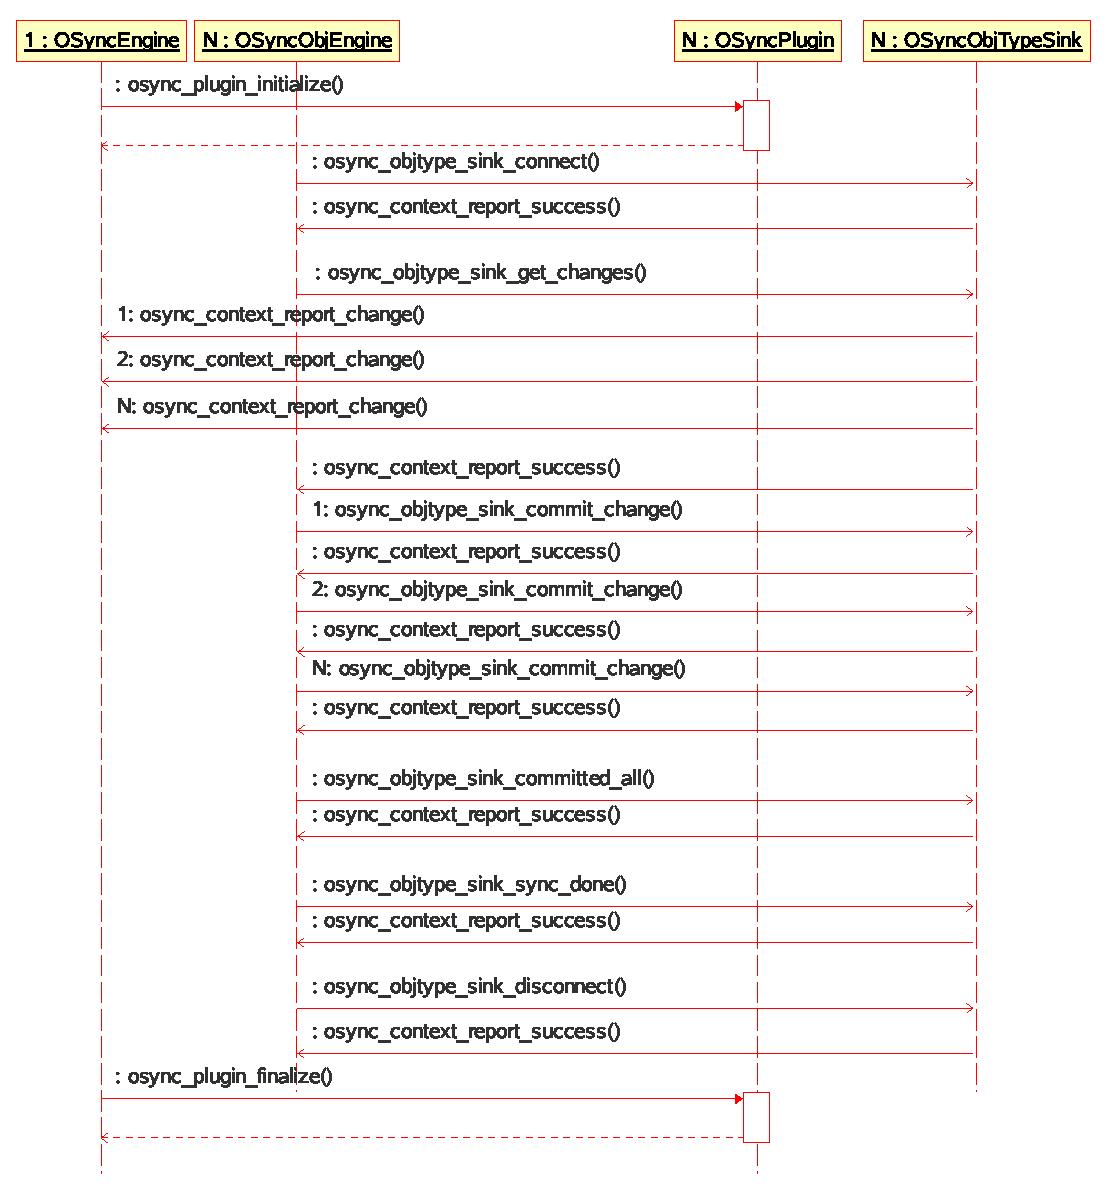
\includegraphics[bb=0 0 661 960, scale=0.60]{simple-sync-sequence}
 % simple-sync-sequence.png: 661x960 pixel, 72dpi, 23.32x33.87 cm, bb=0 0 661 960
 \caption{Plugin Synchronization Sequence}
 \label{fig:SimpleSyncSequence}
\end{figure}

Those function are called "Generic Functions" and MUST be implemented by 
plugin.

\section{Generic Functions}
The Generic Functions are the only functions, which got called synchronously by 
the OpenSync Framework.
\subsection{Initialization}
\subsection{Finalize}
\subsection{Discover}
%\subsection{Usable}
\section{Sink Functions}
All ">Sink Functions"< are called asynchronously, not like the "Generic
Functions", and have to reply with OSyncContext functions if the task was 
executed or not. It's very important that the ">Sink Functions"< reply the
request by the OpenSync Framework with the OSyncContext functions. Even on
error condition the Sink Function have to reply with a special OSyncContext
error function. Otherwise the OpenSync Framework until the timeout for this
function call is reached, which may take sometime for some usually time 
consuming functions\\
The Main Sink, which is Object Type neutral, doesn't have any required Sink 
Functions. For the Object Type Sink are the implementation of some Sink 
Functions required:

\begin{center}
% use packages: array
\begin{tabular}{ll}
\textbf{Function} & \textbf{Implementation} \\ 
Connect & O \\ 
Get Changes & M \\ 
Commit / Batch Commit & M (only Commit \textbf{or} Batch Commit) \\ 
Committed All & O (only available in combination with Commit)\\ 
Synchronization Done & O \\ 
Disconnect & O
\end{tabular}
\end{center}

The Plugin don't have to register a Main Sink if there is no need for Object 
Type neutral tasks.
\subsection{Connect}
The Connect function is available for all Object Type Sinks and could be used to
establish Object Type specific connection. If the connection establishment is an
Object Type neutral task (e.g. Bluetooth, USB, ...) and needded to be done only
once, only the Main Sink should be used. This avoids problems with shared access
to an interface, since a connect function would be called for each Object Type
for the same interface.\\
This function MUST only establish a connection to the device or ressource. After
the connection got established successful the plugin MUST reply the context with
\verb|osync_context_reply_success()|. On error the plugin replies a 
human-readable
(aka. userfriendly) error message with \verb|osync_context_reply_error()|.
\subsection{Get Changes}
The Get Changes function get called by the OpenSync Framework to request changes
since last synchronization or all entries of the Object Type specific ressource.
Later one MUST be done when a Slow Sync got requested by the OpenSync
Synchronization framework. If a Slow Sync got requested for this Sink MUST be
checked with \verb|osync_objtype_sink_get_slowsync()|. On a Slow Sync the 
Changetype (for all changes) is \verb|OSYNC_CHANGE_TYPE_ADDED|. On a regular 
(fast sync) synchronization it's up to the Get Changes function to determine 
the Changetype. Every change have to be reported with 
\verb|osync_context_report_change()|. On a error the Sink Function have to 
reply the context with \verb|osync_context_report_error()| and stop/leave this 
function ASAP. If the protocol, application or device isn't able to report 
changed entries since last sync, the OpenSync Helper Hashtable should be used 
to determine the Changetype of the entry.
\subsection{Commit}
This function get called with a single OSyncChange object, which MUST be
committed to the application or device. If the commit failed the context MUST be
replied with \verb|osync_context_report_error()|. On success the context get 
replied with \verb|osync_context_success()|. If Hashtable is already involved in
the Get Changes functions, then the Commit function has to update the entries 
for the Hashtable for entries which get committed.
\subsection{Batch Commit}
The batch commit function is intended for protocols, device or application which
only allow batch committing (sending all changes at once). This function get
called with an array of changes which have of be committed all at once.
\subsection{Committed All}
This function got called after all entries got committed, even if error appeared
while committing. This function get not called if Batch Commit function is
registered for this Sink.
\subsection{Synchronization Done}
This function got called only after a successful synchronization.
When using Hashtable \verb|osync_hashtable_save()| should get called, to
do persistent store of the Hashtable.
\subsection{Disconnect}
This function MUST only handle the disconnect of the sink. Don't do further
cleanup here, the finalize function is intended for releasing memory and
cleanup. The disconnect function might never get called when even the connect
function failed.
\section{Properties}
Each Synchronization Plugin has properties which get set within the
\verb|get_sync_info()| function. The properties are:

\begin{itemize}
\item Name, short name of the plugin should be less then 15 characters. This
name isn't visible to the user, at least not for rich OpenSync Frontends.
\item Longname, is the name of the plugin which is visible to the user in
rich OpenSync frontends. Should not be longer then 50 characters.
\item Description, about the Plugin visible to the end user in OpenSync
Frontends, and should additionally help to choose the right plugin.
\item Configuration Type, defines if the plugins needs any configuration or if
the configuration is optional or simply not needed.
\item Process Type, defines how the plugin get started: threaded, forked or by 
an external process.
\item Timeouts, for initialization, finalization and timeout can be configured
for the plugin needs. 
\end{itemize}

\subsection{Name}
The name of the plugin get defined like all plugin properties in
\verb|get_sync_info()| function with calling \verb|osync_plugin_set_name()|.
This name got used mostly for internal configuration and isn't visible to the 
user (at least not for rich OpenSync Frontend user). The name should be less
then 15 characters and should one word (no spaces). Example: ">palm-sync"<
\subsection{Longname}
The Longname of the plugin is the only name visible for  regular user to choose 
the correct plugin from a list of available plugins. Use the description field
to describe the plugin in more detail. Don't include the term ">Plugin"> in the
Longname. Example: ">Palm Device"<
\subsection{Description}
The description should additionaltly help the user to choose the correct plugin
if there are several plugins with similar names. Bad example: ">Plugin to sync 
your pda. Version 0.23. http://foo.edu/hacking/opensync"<. The term ">Plugin"< 
might confuse regular user, avoid it. If your plugin supports several different
devices don't list all known to work models, this might confuses people as well.
Again, don't list models! If your plugin is based on a synchronization 
implementation mention the name of protocol. No version numbers, no URLs and 
most user won't care about the authors name or E-Mail address.
\subsection{Plugin Timeouts}
The default plugin timeout should basically fit the need for all plugins. If
your plugin is known to be very slow you can change the timeout for this plugin
with following functions:
\begin{itemize}
\item \verb|osync_plugin_set_initliaze_timeout()|
\item \verb|osync_plugin_set_finalize_timeout()|
\item \verb|osync_plugin_set_discover_timeout()|
%\item \verb|osync_plugin_set_useable_timeout()|
\end{itemize}
The timeout unit is in seconds. It's possible to overwrite custom plugin timeout
with setting individual timeouts in the member configuration (syncmember.conf).
\subsection{Configuration Types}
If the plugin doesn't need any configuration by the user the plugin should the
configuration type to \verb|OSYNC_PLUGIN_NO_CONFIGURATION| with the
\verb|osync_plugin_set_config_type()| function. If the plugin don't need by
default a configuration but could be is additionally configurable the
configuration type should be set to \verb|OSYNC_PLUGIN_OPTIONAL_CONFIGURATION|. 
If the plugin can't perform without any configuration the type should be set
to\\ \verb|OSYNC_PLUGIN_NEEDS_CONFIGURATION| (set by default).
\subsection{Process Types}
The Process Type declares how a plugin get started. By default the plugin get
started by the OpenSync Framework within a thread (
\verb|OSYNC_START_TYPE_THREAD|). If the Plugin is known to conflict with the 
process mainloop of the OpenSync Framework, it's possible to run the plugin in 
a separated process by forking it. The forking is done by the OpenSync
Framework when the start type got set to \verb|OSYNC_START_TYPE_PROCESS|. If the
plugin has to access a not public interface to get access to the data ressources
of an application it's possible to integrate the plugin within this application.
So the plugin is running all the time this application is running and can
communicate with the OpenSync Framework when the Process Type got set to 
\verb|OSYNC_START_TYPE_EXTERNAL|. The Process Type can be changed with the 
\verb|osync_plugin_set_start_type()| function. 
\section{Configuration}
